% Subsystem report for Datapath control system, typeset for the LaTeX processor.
% Copy the next line and put your initials instead of JL.
\fancyfoot[R]{MM}
\section [Power]{Power Subsystem}
\subsection{Description}

The power system \index{power} provides reliable, standalone power to all other hardware subsystems. The design supports three different voltage levels as the ATMEGA8518 MCU, analog signal conditioner, and WT32 bluetooth module all require different reference voltages. The source has the flexibility to operate from battery or, when interfaced with a standard USB port, charge the in-system battery and provide uninterrupted power when switching between the two.  

\subsection{System Power Requirements}

Each subsystem requires a different supply voltage as shown in Table \ref{tab:power requirements}. 
\begin{table}[bhp]
\caption[Power Requirements]{Recommended DC operating voltages for ATMEGA8515\cite{ds:ATMEGA8515} and WT32\cite{ds:WT32}}
\small
\begin{center}
\begin{tabular}{l| c c}
\setlength{\tabcolsep}{1pt}
	Device     & Minimum   & Maximum \\\hline
	ATMEGA8515 & 2.7 V     & 5.5 V   \\             
	Analog Signal 
	Conditioner& -12 V     & +12 V\\            
  \small{ADC}& N/A		   & Quiet 3 V\\
	WT-32      & 2.5 V     & 4.4 V            
\end{tabular}
\end{center}
\label{tab:power requirements}
\end{table}

\subsection{Battery}

Taken into consideration are three potential in-system, rechargeable battery\index{battery} supply options: Alkaline, NiMH, or Li-Poly. For some of the basic metrics taken into consideration see table \ref{tab:battery comparison}. Alkaline batteries in series are not a bad option as it would provide the 3V DC source necessary for the MCU and a similar arrangement could provide power for the other sub-systems as well. The issue with this approach is efficient in-system charging. As with all of the rechargeable batteries considered, use of multiple-cells in a charging system require some intelligent monitoring of each cell to assure that no cell is too far out of sink which can result in overcharging or reverse-charging as a charged cells will rapidly discharge into the uncharged cell. Overcharging can, at the least, damage the battery if not resulting in a dangerous explosion due to an un-containable build up of gaseous bi-products. Another drawback to Alkaline is that voltage output degrades linearly over time which is unfavorable for high-drain electronics. 

NiMH batteries maintain a more consistent voltage over time but have a relatively low efficiency. The best battery solution for this design is the Li-Poly as it not only has a superior efficiency, a single cell outputs a nominal voltage of 3.7 V DC which is acceptable for directly powering the WT-32 bluetooth module. As an added bonus, the WT-32 has a built-in battery charging application as it is often utilized with integrated single cell Li-Poly batteries (i.e. - bluetooth headsets, cell phones). 
  
\begin{table}[bhp]
\caption[Common Battery Types]{Comparison of Common Battery Types\cite{web:bat_tech}}
\small
\begin{center}
\begin{tabular}{l| c c c}
\setlength{\tabcolsep}{1pt}
	Battery     & Single Cell Voltage   & Efficiency & No. of Cycles\\\hline
	Alkaline & 1.5 V                    & 99.9\%        & 100 - 1000\\             
	NiMH     & 1.2 V                    & 66.0\%        & 1000      \\            
  Li-Poly  & 3.7 V		                & 99.8\%        & 500 - 1000 
\end{tabular}
\end{center}
\label{tab:battery comparison}
\end{table}

\subsection{DC/DC Converter}

The Li-Poly battery integrated with the WT32 bluetooth module provides a level 3.7 V DC source which must be re-leveled and distributed to the other sub-systems with as little ripple as possible. Component selection for this application takes into consideration the need for high efficiency. DC-DC converter packages are cheap and readily available so the alternative of building a custom supply is unnecessary. Low-power DC DC converters come in two basic varieties: fixed and adjustable. The adjustable converters feature a built-in gain setting resistor for the internal op-amp and in the case of the LT1073, only three passives are required to configure the device.\hline 


\begin{figure}[hbp]
\centering
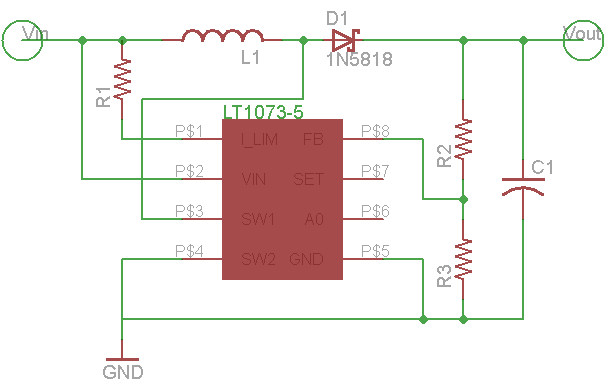
\includegraphics[scale=0.5]{power_gen_fixed.png}
\caption[LT1073 Fixed Output Configuration]{LT1073 general fixed output configuration\cite{ds:lt1073}}
\end{figure}
